\chapter{Contribution} \label{chapter:contribution}
\section{Idea and Motivation}
\paragraph{}
In the previous chapter, the work of Kevin Coogan and Saumya Debray, presented in the paper titled \textit{Equational Reasoning of x86 Assembly Code}~\cite{coogan2011equational}, has been discussed. In the frame of their work, they needed a tool to assist them with analysing traces of Intel x86 instructions from malware. They then put forward a set of rules to translate instructions into equations, and a term-rewriting system to manipulate them. Even if the tool has not been made public, one could write its own version of it for the pseudo code has been published in Kevin Coogan's PHD thesis~\cite{coogan2011deobfuscation}.

\paragraph{}
The contribution of this work will be to show how to extend their tool by allowing it to work in a static analysis context. The authors broadly discussed this idea in the penultimate section, but without diving in depth in the topic. They proposed to turn the assembly code into an intermediate language of type Static Single Assignment, or SSA for short, and they pointed toward a paper to solve the problem of aliasing which comes with indirect memory accesses. In the following sections of this chapter, it will be given a description of the procedures that are required to make their ideas practical for static analysis.

\section{Complications}
\subsection{Branching}
\paragraph{}
In the dynamic analysis case, the various definitions a variable can have are uniquely differentiated by the order number of the defining instruction. Because traces contain the sequence of instructions that have been executed by the CPU in a sequential order, there will not be any branching, or in another words, there will not be the possibility to go back up in the trace. As a result, it is enough to use the order number as a source for unique identifiers. 

\paragraph{}
This is in contrast with the static analysis case, where listings of instructions can contain conditional and unconditional branching instructions. The problematic situation appears when branching toward a part of the listing that has already been seen. It would be necessary to redefine some of the definitions that are used as source operands in between the landing point and the branching instruction to account for the changes of state that have happened during the previous pass. This is in contradiction with the non mutating state property that is essential to the equational reasoning.

\paragraph{}
In Listing~\ref{lst:with_without_branching}, this phenomenon can be observed. To be noted that, for the sake of the example, the two notations have been mixed and the code itself does not serve any purpose. For the new state of $eax$ to be reflected when going back up, one would have to add a definition in the form of $eax_{30} := eax_{31}$ between the equations at line 31 and 32. \\

\begin{lstlisting}[caption={Example where the branching instruction disrupt the analysis.}, label={lst:with_without_branching}, frame=tlrb, language={[x86masm]Assembler}]
<@$ 30: eax_{30} := ebx_{29} + eax_{28} $@>
<@$ 31: eax_{31} := eax_{30} - 1 $@>
<@$ 32: jz\ 30 $@>
\end{lstlisting}

\paragraph{}
In a static analysis situation, one can actually only use the equational reasoning tool of Kevin Coogan and Saumya Debray on basic blocks. Since they are sequences of instructions with no branches getting in except for the entry point, and no branches going out except for the last instruction, the definitions will not have to mutate.

\subsection{Indirect Memory Access} \label{sec:pb_indirect_memory_access}
\paragraph{}
The other issue, which is inherently linked with static analysis, is having indirect memory accesses, that is, having one of the operands of an instruction being a memory expression that has to be computed first. The Intel x86 instructions able to access memory locations are given operands that point to these locations by means of the addressing mode shown in Equation~\ref{eq:addressing_modes}. The brackets indicates optional parameters, at least one of the three brackets has to be used. When dealing with traces, the values of the registers are well known and so, it is easy to find out which memory location is being accessed and or modified. On the contrary, in a static context, it is not always possible to gain this knowledge for registers' values could only be known at runtime. 

\begin{equation} \label{eq:addressing_modes}
\begin{Bmatrix}
CS: & \\ 
DS: & \\ 
SS: & \\ 
ES: & \\ 
FS: & \\ 
GS:
\end{Bmatrix}
\begin{bmatrix} 
	\begin{Bmatrix} 
	EAX & \\ 
	EBX & \\ 
	ECX & \\ 
	EDX & \\ 
	ESP & \\ 
	EBP & \\ 
	ESI & \\ 
	EDI
	\end{Bmatrix}  
\end{bmatrix} + 
\begin{bmatrix} 
\begin{Bmatrix} 
EAX & \\ 
EBX & \\ 
ECX & \\ 
EDX & \\ 
EBP & \\ 
ESI & \\ 
EDI
\end{Bmatrix} *
\begin{Bmatrix} 
1&\\ 
2&\\ 
4&\\ 
8
\end{Bmatrix}
\end{bmatrix} + [displacement]
\end{equation}

\paragraph{}
The equational reasoning relies on the fact that the dependencies between definitions and usages can be traced by simply going upward in the trace. When encountering an operand which is a memory location that has to be dynamically computed, it might not be possible to correctly resolve further dependencies because of unknown aliasing relationships with that operand.

\paragraph{}
An example can be observed in Listing~\ref{lst:indirect_memory_access_example}. In this scenario, the registers $ebp$ and $esp$ are pointing toward the same memory location. Both registers are marked as constant for the sake of the example. The first and second lines are setting the same location in memory to a different value, the third line is using the value stored in the memory location to perform an exclusive or. Because the algorithm which performed the translation into the equational form did not realised $[ebp]$ and $[esp]$ were aliased, it uses the old value, $42$, as one of the two operands of the exclusive or. As a result, the translation algorithm produced an erroneous listing. \\

\begin{lstlisting}[caption={Example of a problematic situation that arose from indirect memory accesses.}, label={lst:indirect_memory_access_example}, frame=tlrb, language={[x86masm]Assembler}]
<@$ ValueAt(MLOC[esp_{cons}..esp_{cons}+3])_1 := 42 $@>
<@$ ValueAt(MLOC[ebp_{cons}..ebp_{cons}+3)])_2 := 43 $@>
<@$ eax_3 := eax_{cons} \oplus ValueAt(MLOC[esp_{cons}..esp_{cons}+3])_1 $@>
\end{lstlisting}

\section{Static Single Assignment}
\paragraph{}
Static Single Assignment is a property a language can have. It states that each variable can only be assigned once. As a consequence, languages with this property are referentially transparent. Indeed, if a variable cannot be reassigned, states cannot mutate. Andrew W. Appel even argues in his paper titled \textit{SSA is Functional Programming}~\cite{appel1998ssa}, that, without too many surprises, SSA is indeed functional programming. 

\paragraph{}
One might have noticed that the language presented in the previous chapter is in SSA form. Each variable definition is assigned a unique identifier which is the line where the original instruction appears in the trace, and each uses of a variable is renamed to match the definition's new name. 

\paragraph{}
Languages based on SSA are widely used by compilers to perform optimisations such as constant propagation~\cite{wegman1991constant}, code motion~\cite{click1995global}, and elimination of partial redundancies~\cite{briggs1994effective} because it is a very efficient way of representing the data flow of programs. They operate as follows: First a source code is turned into an SSA form, then the SSA form is applied to as many optimisation algorithms as possible, and finally the SSA form is translated back into either the source language or another language.

\paragraph{}
The SSA form has been introduced by Ron Cytron et al in the paper titled \textit{Efficiently Computing Static Single Assignment Form and the Control Dependence Graph}~\cite{cytron1991efficiently} published in 1991. The efficient algorithm they proposed to turn a program into an SSA form requires a control flow graph as input. In a reverse engineering context, this is just what one would want for most tools provide this representation by default. 

\paragraph{}
Contrary to the representation of Kevin Coogan and Saumya Debray, the SSA form provides a way to follow the dependencies when dealing with branching. It is done thanks to the $\phi$-function, which is a special kind of assignment that takes two or more definitions of the same variable and turns them into a new definition. This can be observed in Listing~\ref{lst:phi_function}. Because of the $do$/$while$ construct, the $x:=x*2$ statement can be executed more than once, and so requires special care. The semantic of the $\phi$-function is that, if the control flow comes from the first assignment, $x_2$ will be equal to $x_1$, and if the control flow comes from the loop construct, $x_2$ will be equal to $x_3$. \\ \\

\noindent\begin{minipage}{.45\textwidth}
	\begin{lstlisting}[caption={A simple while loop}, label={lst:before_phi_function}, frame=tlrb, language=C]
<@$ x := 1 $@>
<@$ do $@>
<@$ \qquad x := x * 2 $@>
<@$ while\ P $@>
	\end{lstlisting}
\end{minipage}\hfill
\begin{minipage}{.45\textwidth}
	\begin{lstlisting}[caption={Translating a while loop found in Listing~\ref{lst:before_phi_function} into a SSA form using a $\phi$ function.}, label={lst:phi_function}, frame=tlrb, language=C]
<@$ x_1 := 1 $@>
<@$ do $@>
<@$ \qquad x_2 := \phi(x_1, x_3) $@>
<@$ \qquad x_3 := x_2 * 2 $@>
<@$ while\ P $@>
	\end{lstlisting}
\end{minipage}

\paragraph{}
The remaining parts of this section will be about defining more formally the notion of control flow graph, and then giving the procedure to translate code into a SSA form.

\subsection{Control Flow Graph}
\paragraph{}
A CFG is a directed graph whose nodes are basic blocks and where edges represent the transfer of control between these blocks. To be complete, two more nodes are added: The entry node that connects every basic block from which the program can be entered, and the exit node which is connected to every block that can exit the program. In this configuration, every node is on at least one path from Entry and one path to Exit. Each variable used in any of the basic block has been initialised in the Entry block to whatever value which may represent the starting state of these variables.

\paragraph{}
An edge from the block $X$ to the block $Y$ will be represented by $X\rightarrow Y$. The successors of a node $X$ are every node $Y$ with an edge $X\rightarrow Y$. The predecessors of a node $X$ are every node $Z$ with an edge $Z\rightarrow X$. The set of all successors of a node $X$ will be then represented by $Succ(X)$, and the set of all predecessors by $Pred(X)$. A joint node is a node that has more than one predecessor.

\paragraph{}
A non-null path from node $X_0$ to node $X_j$ of size $J$ will be denoted as $X_0 \stackrel{+}\rightarrow X_j$. Two non-null paths $X_0\stackrel{+}\rightarrow X_j$ and $ Y_0\stackrel{+}\rightarrow Y_k$ converge at node $Z$ if:
\begin{gather*} 
X_0 \neq Y_0 \\
X_j = Z = Y_k \\
(X_j = Y_k) \implies (j = J\ or\ k = K)
\end{gather*}
Intuitively, two non-null paths converge if they join at the end.

\subsection{Translating into SSA form}
\paragraph{}
According to Cytron et al~\cite{cytron1991efficiently}, a program is in an SSA form if it meets these three conditions:
\begin{itemize}
	\item \textbf{First condition}: Two non-null paths $X\stackrel{+}\rightarrow Z$ and $Y\stackrel{+}\rightarrow Z$ converge at a node $Z$, and nodes $X$ and $Y$ contain assignment to $V$ in the original program, then a trivial $\phi$-function $V\leftarrow \phi(V, ..., V)$ has been inserted at $Z$ in the new program.
	\item \textbf{Second condition}: Each mention of $V$ in the original program or in an inserted $\phi$-function has been replaced by a mention of a new variable $V_j$, leaving the new program in SSA form.
	\item \textbf{Third condition}: Along any control flow path, consider any use of a variable V in the original program and the corresponding use of $V_i$ in the new program. Then $V$ and $V_i$ have the same value.
\end{itemize}
	
\paragraph{}
Translating a program into an SSA form is then done in two steps: 
\begin{itemize}
	\item \textbf{First step}: It consists of inserting trivial $\phi$-functions at the entrance of certain join nodes in the CFG. They will have the following form: $V \leftarrow \phi(W, X, ..)$. The amount of operands applied to the $\phi$-function will depend on how many predecessors the node has. The predecessors will be listed in a fixed order, and the $j$th operand of $\phi$ will be associated with the $j$th predecessor. This simply means that, if the control flow comes from the $j$th node, the $j$th operand will be selected by the $\phi$-function.
	\item \textbf{Second step}: It consists of replacing each mention of a variable $V$ by a new variable $V_j$ so that the three properties stated above hold.
\end{itemize}

\paragraph{}
An SSA form which has a minimal amount of $\phi$-functions, while keeping the first condition true, is said to be in minimal SSA form. Another flavour of SSA is called pruned SSA~\cite{choi1991automatic} form, and has the particularity of not having $\phi$ function for variable that are not live in the rest of the program. In our situation, we want the minimal form so that we can analyse the data flow of a variable at any point in the code. The steps to turn a program into a minimal SSA form will then be described in the following sections.

\subsubsection{Setting the $\phi$-functions}
\paragraph{}
A naïve approach to finding out where to put the $\phi$-functions would be to enumerate every pairs of assignment for the same variable and verify if they can reach a common node. The problem with this method is that it is not something that can be achieved in linear time. Another way to find out where to make the insertions is to use the dominance frontier of every node.

\paragraph{}
Before explaining what is a dominance frontier, it is first necessary to lay down a little bit of terminology.
\begin{itemize}
	\item For two nodes $X$ and $Y$ from a CFG, it is said that $X$ dominates $Y$ if $X$ is on every path from the Entry node to $Y$. This relationship will be denoted as follows: $X \geq Y$.
	\item If $X$ dominates $Y$ and $X\neq Y$, it is said that $X$ strictly dominates $Y$. This relationship will be denoted as follows: $X > Y$.
	\item If $X$ does not strictly dominate $Y$, the following notation will be used: $X \ngtr Y$.
	\item The immediate dominators of a node $X$ are the closest strict dominators of $X$ on the paths from Entry to $X$ on the CFG. A node can have more than one immediate dominators. The set of all immediate dominators of a node $X$ will be denoted as follows: $idom(X)$.
	\item $Dom(X)$ represents the set of all nodes that dominate $X$.
\end{itemize}

\paragraph{}
The dominance frontier of a node $X$ is the set of all nodes $Y$ that are not strictly dominated by $X$ while having at least one successor which is dominated by $X$. More formally, the dominance frontier can be defined as:\\
\begin{gather*} 
DF(X) = \left\{Y\ |\ \exists P \in Pred(Y),\ X \geq P\ and\ X \ngtr Y\right\}
\end{gather*}

\paragraph{}
To better illustrate the concept of dominance frontier, let's use the CFG found in Figure~\ref{fig:control_flow_graph} as an example. Each node is identified by its number, and, as said before, the entry node initialises every variable to some value to represent the state of the program at its start. Node $4$ dominates nodes $5$, $6$, and $7$. The dominance frontier of node $4$ is then nodes $3$, $10$, and $9$.

\begin{figure}[!htb]
	\centering
	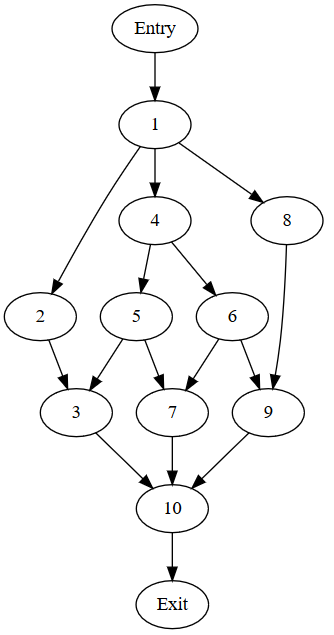
\includegraphics[width=0.35\textwidth]{contribution/graph_example.png}
	\caption{Example of control flow graph which requires $\phi$-functions.}
	\label{fig:control_flow_graph}
\end{figure}

\paragraph{}
In the context of the same example, let's say variable $V$ gets redefined in node $4$. Node $5$, $6$, and $7$ will not need $\phi$-functions for that variable because they will only be exposed to the definition of node $4$. Node $9$, on the other hand, will be exposed to either the definition of the entry node or the definition of node $4$. It then requires a $\phi$-function. 

\paragraph{}
The algorithm used to find out the dominance frontier of every node in the CFG is given in Alg~\ref{alg:dom_front}. As an input, it takes a CFG, but also a dominator tree. The dominator tree is a data structure where each node has for children the nodes it immediately dominates, and where the root node is the entry node. The dominator tree can be computer in linear time with the algorithm presented by Thomas Lengauer and Robert Tarjan in an almost linear time~\cite{lengauer1979fast}. In the algorithm, $Children(X)$ relates to the children of a node in the dominator tree.

\begin{algorithm}
	\begin{algorithmic}[1]
		\For{each $X$ in a bottom up traversal of the dominator tree}
			\State $DF(X) \leftarrow \varnothing$
			\For{each $Y \in Succ(X)$}
				\If{$idom(Y) \neq X$}
					\State $DF(X) \leftarrow DF(X) \cup \left\{Y\right\}$
				\EndIf
			\EndFor
			\For{each $Z \in Children(X)$}
				\For{each $Y \in DF(Z)$}
					\If{$idom(Y) \neq X$}
						\State $DF(X) \leftarrow DF(X) \cup \left\{Y\right\}$
					\EndIf
				\EndFor
			\EndFor
		\EndFor
	\end{algorithmic}
	\caption{Algorithm proposed by Cytron et al~\cite{cytron1991efficiently} to compute the dominator frontier of each node of a CFG.}
	\label{alg:dom_front}
\end{algorithm}

\paragraph{}
And finally, the algorithm to place the $\phi$-functions is given in Alg~\ref{alg:phi_function}. $Work(*)$ and $HasAlready(*)$ are arrays of flags, and $A(V)$ is the set of nodes which contain an assignment to $V$. For the proof of correctness of these two algorithms, as well as their complexity analysis, one should refer to the authors' paper~\cite{cytron1991efficiently}.

\begin{algorithm}
	\begin{algorithmic}[1]
		\State $IterCount \leftarrow 0$
		\For{each node $X$ do}
			\State $HasAlready \leftarrow 0$
			\State $Work \leftarrow 0$
		\EndFor
		\State $W \leftarrow \varnothing$
		\For{each variable $V$}
			\State $IterCount \leftarrow IterCount + 1$
			\For{each $x \in A(V)$}
				\State $Work(X) \leftarrow IterCount$
				\State $W \leftarrow W  \cup \left\{X\right\}$
			\EndFor
			\While{$W \neq \varnothing$}
				\State Take $X$ from $W$
				\For{each $Y \in DF(X)$}
					\If{$HasAlready(Y) < IterCount$}
						\State place $V \leftarrow \langle\phi(V, ..V)\rangle$ at $Y$
						\State $HasAlready(Y) \leftarrow IterCount$
						\If{$Work(Y) < IterCount$}
							\State $Work(Y) \leftarrow IterCount$
							\State $W \leftarrow W \cup \left\{y\right\}$
						\EndIf
					\EndIf
				\EndFor
			\EndWhile
		\EndFor
	\end{algorithmic}
	\caption{Algorithm proposed by Cytron et al~\cite{cytron1991efficiently} to insert the $\phi$-functions.}
	\label{alg:phi_function}
\end{algorithm}


\subsubsection{Variable Renaming}
\paragraph{}
First of all, it is necessary to give the form the assignments will obtain in the SSA form. An assignment A will be turned into $LHS(A) \leftarrow RHS(A)$, where $LHS(A)$ is a tuple of distinct variables, and where $RHS(A)$ is a tuple of expressions. Obviously, it is required for these two tuples to be of equal size for the variables get assigned to the value of the expressions. The use of tuple is necessary for constructs such as function calls, where multiple variables can be defined at the same time.

\paragraph{}
It is also required to describe the data structure which will be used by the algorithm: $C(*)$ is an array of integers which records how many assignments every variable has been exposed to so far, $S(*)$ is an array of stacks, one per variable, which contains integers, and where the top of the stacks contains the value $i$ used to construct the variables, $WhichPred(X, y)$ is an integer that represents which predecessor of $Y$ in the CFG $X$ is, and $oldLHS(a)$ is the original tuple.

\paragraph{}
The algorithm for renaming can be observed in Alg~\ref{alg:rename}. It begins by initialising $C(*)$ and $S(*)$, and then it starts a top down traversal on the dominator tree, beginning with the $entry$ node. This can be observed between line 1 and line 5. The search function will handle the renaming. Its first loop will do the renaming of the $RHS$ variables which are not part of a $\phi$-function, and every $LHS$ variable. This can be observed between line 8 and line 20. The next loop, between line 21 and line 26, will handle the renaming of the $RHS$ variables that are part of a $\phi$-function. The recursive descent is handled between line 27 and line 29. Finally, some bookkeeping is done between line 30 and line 34.

\begin{algorithm}
	\begin{algorithmic}[1]
		\For{each variable $V$}
			\State $C(V) \leftarrow 0$
			\State $S(V) \leftarrow EmptyStack$
		\EndFor
		\State \MCall $search(Entry)$
		\State
		\Function{search}{$X$}
			\For{each statement A in X}
				\If{$A$ is an ordinary assignment}
					\For{each variable $V$ used in $RHS(A)$}
						\State replace use of $V$ by use of $V_i$, where $i = Top(S(V))$
					\EndFor
				\EndIf
				\For{each $V$ in $LHS(A)$}
					\State $i \leftarrow C(V)$
					\State replace $V$ by new $V_i$ in $LHS(A)$
					\State push $i$ onto $S(V)$
					\State $C(V) \leftarrow i + 1$
				\EndFor
			\EndFor
			\For{each $Y \in Succ(X)$}
				\State $j \leftarrow WhichPred(Y, X)$
				\For{each $\phi$-function $F$ in $Y$}
					\State replace the $j$-th operand $V$ in $RHS(F)$ by $V_i$ where $i = Top(S(V))$
				\EndFor
			\EndFor
			\For{each $Y \in Children(X)$}
				\State \MCall $search(Y)$
			\EndFor
			\For{each assignment $A$ in X}
				\For{each $V$ in $oldLHS(A)$}
					\State $pop S(V)$
				\EndFor
			\EndFor
		\EndFunction
	\end{algorithmic}
	\caption{Algorithm proposed by Cytron et al~\cite{cytron1991efficiently} to rename the variables.}
	\label{alg:rename}
\end{algorithm}

\subsection{Memory Aliasing} \label{sec:memory_aliasing}
\begin{quotation}
	\noindent ``\emph{As a result of alias issues, memory expressions must be divided into those which are safe to propagate, and those which must not be propagated at all.}''
	\begin{flushright}\textbf{Michael James Van Emmerik, 2007}\end{flushright}
\end{quotation}

\paragraph{}
As explained before in Section~\ref{sec:pb_indirect_memory_access}, the indirect memory accesses cause problems in a static context for it is not easy to follow the data flow, and as a result, propagating values gets tricky. This is due to the fact that there is more than one way to refer to the same memory location. The causes of these aliasings are mostly from the manipulation of the stack, and the frame pointers~\cite{van2007static}. Fortunately, there cannot be such aliasing problems with registers. Indeed, the only way to change the content of, or to refer to content of, let's say, $eax$ is to explicitly specify $eax$, or one of its three other names, as an operand.

\paragraph{}
One of the many solutions would be the following: Heap storage can be modelised as one single variable that is redefined every time one of its region is updated. This approach is not very conservative but still allows optimization to be done~\cite{cytron1991efficiently}. Unfortunately, in our context, we do not only want to apply optimisation, but also to provide a way to follow the data flow in certain regions of the program. 

\paragraph{}
Another solution would be to not propagate $LHS$ variables that are defined by functions which are applied to at least one memory expression, but this is not what one would want to have. Propagation is possible, easily inside basic blocks, and in a more complicated way across basic blocks.

\paragraph{}
As said before, one could reason about memory locations from within a basic block. Two memory locations $i$ and $j$ are non conflicting if at least one of the two following conditions hold:
\begin{itemize}
	\item The memory location $i$ uses a register known to point to the stack, while the memory location $j$ points to the heap. 
	\item They use the same base register but different offset, and the base register is not redefined in between the two memory locations.
\end{itemize}
This is again not enough for we want something which allows data to be followed outside basic blocks.

\paragraph{}
A third solution, one that would be satisfactory, is the one proposed by Gogul Balakrishnan et al in the paper titled \textit{Analyzing Memory Accesses in x86 Executables}~\cite{balakrishnan2004analyzing}. In it, they describe a static analysis algorithm for x86 executable files called the \textit{value-set analysis}, which yields an over approximation of the set of values each data object can hold at each program point. A data object can either be a memory location or a register. To modelise the data objects, they introduced the concept of abstract locations, or a-locs for short. Intuitively, an a-loc can be roughly compared to a variable in a programming language such as $C$. More precisely, a-locs are based on the fact that generating an executable from a high level language comes after establishing the data layout of the program: Global variables will be accessed through static addresses, and local variables will be accessed through static stack frame offsets that are added or subtracted to either $esp$ or $ebp$. An a-loc is simply a set of locations between two statically known locations/offsets. To be noted that they thus cannot overlap.

\paragraph{}
To illustrate the results the value-set analysis would give, let's use the example provided in the paper~\cite{balakrishnan2004analyzing}. It is not an original one for the tool performing the analysis is not freely available. The original C code can be found in Listing~\ref{lst:vsa_c}, its assembly version can be found in Listing~\ref{lst:vsa_asm}. To be noted that the C code is not used by the value-set analysis and has only been added to make the example easier to understand from the reader's perspective. The purpose of the code is to fill the first half of the $a$ array with $0$s, to fill the other half with $1$s, and finally to return the first value of $a$. Upon inspection of the assembly code, one would notice that variables $part1$, $part2$, and $i$ have been replaced by registers, respectively $eax$, $ebx$, and $ecx$. Also, the two global variables, $part1Value$ and $part2Value$, are stored at addresses $4$ and $8$, respectively. \\ \\


\noindent\begin{minipage}{.45\textwidth}
	\begin{lstlisting}[caption={Sample of C code used for the value-set analysis. This has been taken from the paper of Gogul Balakrishnan et al~\cite{balakrishnan2004analyzing}.}, label={lst:vsa_c}, frame=tlrb, language=C]
int part1Value = 0;
int part2Value = 1;

int main() {
	int *part1, *part2;
	int a[10], *p_array0;
	int i;
	
	part1=&a[0];
	p_array0=part1;
	part2=&a[5];
	
	for(i=0; i<5; i++) {
		*part1=part1Value;
		*part2=part2Value;
		part1++;
		part2++;
	}
	
	return *p_array0;
}
	\end{lstlisting}
\end{minipage}\hfill
\begin{minipage}{.45\textwidth}
	\begin{lstlisting}[caption={Assembly code resulting from the C code found in Listing~\ref{lst:vsa_c}. This has been taken from the paper of Gogul Balakrishnan et al~\cite{balakrishnan2004analyzing}.}, label={lst:vsa_asm}, frame=tlrb, language={[x86masm]Assembler}]
    proc main
1:  sub esp, 44
2:  lea eax, [esp+4]
3:  lea ebx, [esp+24]
4:  mov [esp+0], eax
5:  mov ecx, 0
6:  mov edx, [4]
7:  mov [eax], edx
8:  mov edx, [8]
9:  mov [ebx], edx
10: add eax, 4
11: add ebx, 4
12: inc ecx
13: cmp ecx, 5
14: jl 6
15: mov edi, [esp+0]
16: mov eax, [edi]
17: add esp, 44
18: retn
	\end{lstlisting}
\end{minipage}

\paragraph{}
On the left side of Figure~\ref{fig:data_layout_memory_region}, it can be observed the data layout of the compiled program from Listing~\ref{lst:vsa_c}. The stack frame contains the local variables, being the array of $10$ integers $a$, and $p\_array0$. The two global variables are somewhere else, outside the stack. On the right, one can see the two memory regions that the value-set analysis would detect. Memory regions are continuous parts of the memory space of the program. There is one per memory allocation statement (malloc), one for the global region, and one for each procedure. To be noted that the AR in AR-main stands for activation record, which is another name given to a stack frame. For the value-set analysis, memory addresses are made by a pair memory region-offset. For example, $part1Value$ is located at address $(Global, 4)$.

\paragraph{}
The a-locs of the example can also be observed on the right side of Figure~\ref{fig:data_layout_memory_region}. The a-loc $var\_40$ represents the set of locations between $var\_20$ and $var\_44$, that is, $a[0]$ to $a[4]$ included. The a-loc $var\_44$ represents the set of locations between $var\_44$ and the end of the AR-main region, that is, the end of the stack frame. It maps to $p\_array0$ in the data layout.

\begin{figure}[!htb]
	\centering
	\includegraphics[width=1\textwidth]{contribution/data_layout_and_memory_region.png}
	\caption{Data layout and memory regions of the program found in Listing~\ref{lst:vsa_c}. This has been taken from the paper of Gogul Balakrishnan et al~\cite{balakrishnan2004analyzing}.}
	\label{fig:data_layout_memory_region}
\end{figure}

\paragraph{}
The algorithm over approximates the set of values each a-loc can take, and to represent the over approximation, it uses the notion of reduced interval congruence, or RIC for short. A RIC can be represented as a tuple of $4$ elements, $(a, b, c, d)$, and it means $a*[b, c]+d$. Formally, it denotes the set $\left\{aZ + D | Z \in [b, c]\right\}$. As an example, $(2, 0, 4, 1)$, or $2*[0, 4]+1$, represents the set $\left\{1, 3, 5, 7, 9\right\}$.

\paragraph{}
Finally, the value-set analysis would yield the following result for the entry of main: $\left\{esp \rightarrow (\bot, 0), mem\_4 \rightarrow (0, \bot), mem\_8 \rightarrow (1, \bot)\right\}$. The first element of each tuple that is pointed to by the a-locs corresponds to the global memory region, and the second element corresponds to the AR-main memory region. The results tell us that $esp$ will not have any meaningful values in the global region, and that it will have the value $0$ in the AR-main region. If the analysis was to be run on line $7$, it would yield the following results: 
\begin{equation}
\begin{split}
\left\{ esp \rightarrow (\bot, -44), mem\_4 \rightarrow (0, \bot), mem\_8 \rightarrow (1, \bot), eax \rightarrow (\bot, 4[0,\infty ]-40), \right. \\
\left. ebx \rightarrow (\bot, 4[0,\infty ]-20), var\_44 \rightarrow (\bot, -40), ecx \rightarrow ([0, 4], \bot) \right\}
\end{split}
\end{equation}
If it was run for line $16$, this would have been the results:
\begin{equation}
\begin{split}
\left\{ esp \rightarrow (\bot, -44), mem\_4 \rightarrow (0, \bot), mem\_8 \rightarrow (1, \bot), eax \rightarrow (\bot, 4[1,\infty ]-40), \right. \\
\left. ebx \rightarrow (\bot, 4[1,\infty ]-20), var\_44 \rightarrow (\bot, -40), ecx \rightarrow ([5,5], \bot), edi \rightarrow (\bot, -40)\right\}
\end{split}
\end{equation}

\paragraph{}
Because the analysis determined that $edi$ can take values from the set $\left\{0, 1, 2, 3, 4\right\}$, it is clear that $[eax]$ and $[ebx]$ are not aliased. Reminder that $[eax]$ is $*part1$, and that $[ebx]$ is $*part2$.

\paragraph{}
For more information about the value-set analysis, one should refer itself to the paper~\cite{balakrishnan2004analyzing}. The analysis proposed in it has been implemented in the form of a non-free plug-in for the IDA Pro framework called \textit{CodeSurfer/x86}\footnote{See \url{https://www.grammatech.com/products/codesurfer}.}. At the time of writing, and to the best of my knowledge, it is the only implementation of the value-set analysis.

\section{Implementation and Difficulties}
\paragraph{}
In this section, it will be described how one could implement the tool proposed by Kevin Coogan and Saumya Debray, which has been presented in Chapter~\ref{chapter:equational_reasoning}, to work in a static context. As a reminder, their tool is only able to process traces of x86 assembly code, and so only provides dynamic analysis. Afterwards, the limitations that will suffer the resulting tool will be discussed.

\subsection{Possible Implementation and Difficulties}
\paragraph{}
The tool will take as input an executable file, and it will yield a control flow graph where nodes will be containing code in an SSA form. Moreover, the tool will have to allow analysis of registers and memory locations, as the tool of Kevin Coogan and Saumya Debray can do. To implement it, one can either start from scratch, or build up on top of an existing foundation. The later option will be described.

\paragraph{}
IDA Pro is a reverse engineering framework which has a great reputation in the reverse engineering world. It provides a disassembler, a debugger, but it also provides a scripting engine and a software development kit which allows programmers to extend the capabilities of the tool~\cite{eagle2011ida}. These capabilities and the fact that CodeSurfer/x86 is also a plug-in of IDA Pro, motivated the choice of IDA for the potential implementation of the tool.

\begin{figure}[!htb]
	\centering
	\includegraphics[width=1\textwidth]{contribution/code_surfer.png}
	\caption{Organisation of CodeSurfer/x86. Image inspired from the paper titled \textit{WYSINWYX: What you see is not what you eXecute}~\cite{balakrishnan2010wysinwyx}.}
	\label{fig:codesurfer}
\end{figure}

\paragraph{}
CodeSurfer/x86 is a plug-in for IDA Pro which makes use of the value-set analysis explained in Section~\ref{sec:memory_aliasing}. It is used to generate intermediate representations for x86 programs, which can subsequently be explored through a graphical interface, or through a programming API and its scripting language. Amongst all the things it provides figures a pointer analysis, which allows to see which pointers point to which variables. For more information about its other capabilities, one should refer itself to the official website\footnote{See \url{https://www.grammatech.com/products/codesurfer} again.}. 

\paragraph{}
The architecture of CodeSurfer/x86, and how it interacts with IDA Pro, can be observed in Figure~\ref{fig:codesurfer}. The connector will first create data structures necessary to CodeSurfer/x86 by using the information coming from IDA Pro. The connector then performs the value-set analysis, and it passes information along to CodeSurfer. From CodeSurfer, a programmer can obtain the results of the pointer analysis as well as the control flow graph of the program being analysed using the API, which is accessible both in Scheme and C. The many other functionalities of CodeSurfer are not of interest for this work, and so they will not be discussed. 

\paragraph{}
Finally, if one wants to implement to tool, he or she will have to apply the following operations:
\begin{enumerate}
	\item Get the CFG from IDA Pro, or the one from CodeSurfer.
	\item Get the points-to sets from CodeSurfer.
	\item Go through the points-to sets to clearly identify aliased memory expressions.
	\item Apply the translation from instruction to equations which has been explained in Section~\ref{sec:translating_instructions}, without putting subscripts. Depending on the result of step $3$, additional equations will have to be added to handle aliasing.
	\item Apply the algorithm of Cytron et al~\cite{cytron1991efficiently} to insert the $\phi$-functions. The algorithm can be observed in Alg~\ref{alg:phi_function}.
	\item Apply the second algorithm of Cytron et al~\cite{cytron1991efficiently} to perform the renaming using subscripts. The algorithm can be observed in Alg~\ref{alg:rename}.
	\item Build up the equations for chosen registers and memory locations by simply looking for the latest reaching definitions. This has been explained in Section~\ref{sec:rewriting}.
\end{enumerate}

\paragraph{}
The fourth step mentions that additional equations will have to be added to handle aliasing. Fred Chow et al proposed a way to represent these aliasing relationships in the paper titled \textit{Effective Representation of Aliases and Indirect Memory Operations in SSA Form}~\cite{chow1996effective} by means of, amongst other things, $MayDef$ definitions. This special definition takes as single operand the variable that may be modified, and it gives back another definition of the same variable. It is stated that a MayDef definition only potentially redefine a variable, and so leaves the possibility for the previous definition of that variable to be still referenced. It is modelised by the $\chi$-function, and it could looks like this: $v_x := \chi(v_{x-1})$. 

\paragraph{}
In our case, we would like to also see what is causing the possible redefinition, and so, it would be preferable to add its possible value (or the location containing the value) as a second operand. This can be observed in Listing~\ref{lst:chi_function}. To be noted that $ValueAt$ has been replaced by brackets for readability reasons. In Listing~\ref{lst:no_chi_function}, we know, thanks to previous analysis, that they are referencing to the same exact location for all execution path, and so it is possible to use a more straight forward approach. \\ \\

\noindent\begin{minipage}{.45\textwidth}
	\begin{lstlisting}[caption={The memory location a and b are referencing to the same location.}, label={lst:no_chi_function}, frame=tlrb, language=C]
<@$ [a]_1 := 5 $@>
<@$ [b]_2 := 6 $@>
<@$ [a]_2 := [b]_2 $@>
	\end{lstlisting}
\end{minipage}\hfill
\begin{minipage}{.45\textwidth}
	\begin{lstlisting}[caption={The memory location a and b \textbf{may} be referencing to the same location.}, label={lst:chi_function}, frame=tlrb, language=C]
<@$ [a]_1 := 5 $@>
<@$ [b]_2 := 6 $@>
<@$ [a]_2 := \chi([a]_1, [b]_2) $@>
	\end{lstlisting}
\end{minipage}

\paragraph{}
The difficulties in implementing this tool reside in the fact that IDA Pro and CodeSurfer/x86 are not easily accessible for they need to be purchased, but also because of the amount of work that implementing the algorithm of Kevin Coogan requires. The Intel x86 architecture posses many hundreds of instructions, which should be handled by the translation part of the algorithm. One short-cut would be to only implement the translation for the most common mnemonics. Peter Kankowski has disassembled three popular open-source applications which were compiled with the Microsoft Visual C++ 6.0 compiler, and he displayed the frequency of apparition of each mnemonic in a pie chart. The pie chart can be observed in Figure~\ref{fig:mnemonic_frequency}, and his analysis can be found in the strchr blog\footnote{See \url{https://web.archive.org/web/20151116072930/http://www.strchr.com/x86_machine_code_statistics}.}.

\begin{figure}[!htb]
	\centering
	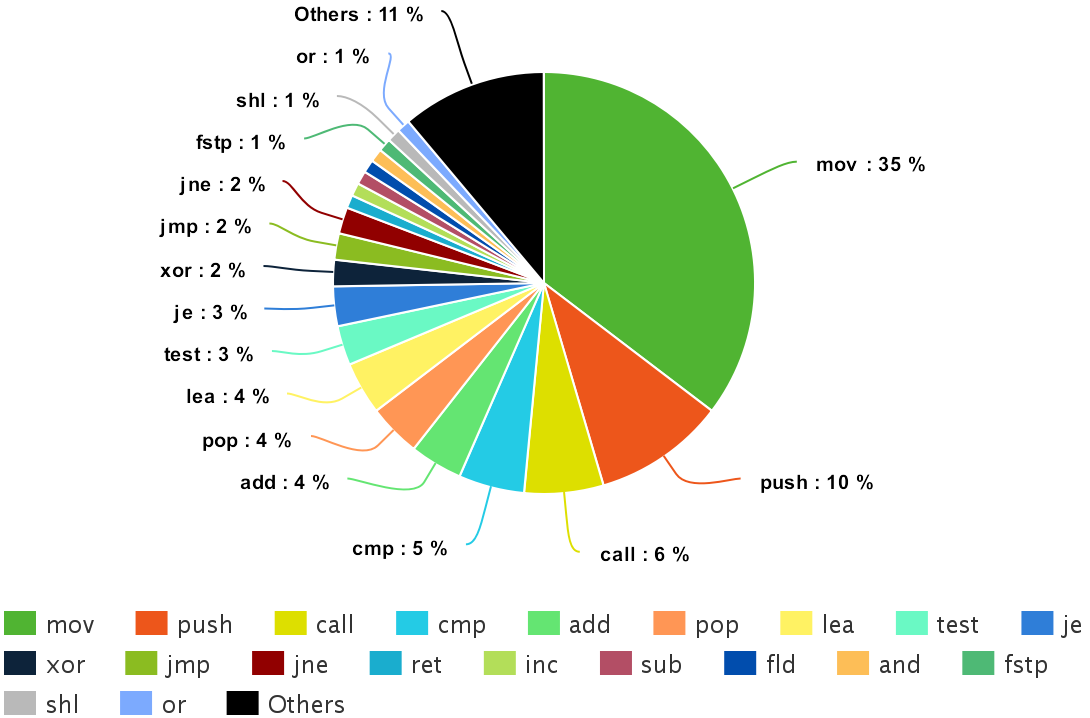
\includegraphics[width=1\textwidth]{contribution/meta-chart.png}
	\caption{Frequency of mnemonic in the Intel syntax. Chart made on \url{https://www.meta-chart.com/}.}
	\label{fig:mnemonic_frequency}
\end{figure}

\pagebreak

\subsection{Limitations}
\paragraph{}
The limitations come from the additions required to make the tool work in a static context. Two problems had to be resolved: Branching, and memory aliasing due to indirect memory accesses. They both come at a price that will be discussed hereunder.

\subsubsection{SSA Form}
\paragraph{}
The SSA form makes use of the $\phi$-functions to handle the redefinitions. These functions will arguably deteriorate the readability of the code, which was one of the arguments used by the authors of the original tool to justify its creation. The example found in Listing~\ref{lst:limitation_asm} will be used to illustrate the point. The code is made of three basic blocks, line $1$ and $2$ being the first one; line $3$, $4$, and $5$ being the second one; and finally, line $6$ being the third one. In this example, a $\phi$-function has to be inserted for $eax$, as seen in the CFG of the SSA form of the code in Figure~\ref{fig:limitation_cfg}. To be noted that the CFG does not include all the equations which interact with $eflags$.\\

\pagebreak

\begin{lstlisting}[caption={Simple assembly code.}, label={lst:limitation_asm}, frame=tlrb, language={[x86masm]Assembler}]
1: mov eax, 0
2: mov ebx, 5
3: add eax, 1
4: cmp eax, 5
5: jz 3
6: add eax, ebx
\end{lstlisting}

\begin{figure}[!htb]
	\centering
	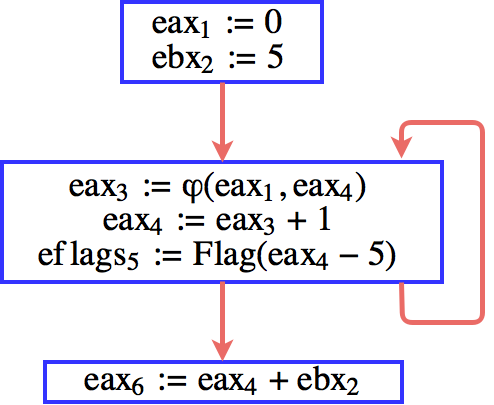
\includegraphics[width=0.6\textwidth]{contribution/limitation_cfg.png}
	\caption{Control flow graph of the SSA form of the code found in Listing~\ref{lst:limitation_asm}.}
	\label{fig:limitation_cfg}
\end{figure}

\paragraph{}
One can notice that the subscripts will not necessarily correspond to the line number of the instructions. For example, line 3 in Listing~\ref{lst:limitation_asm} does not correspond to the equation with a subscript of $3$ in the CFG of Figure~\ref{fig:limitation_cfg}. Also, when substituting the operands with their definition, the $\phi$-function will get in the way. For example, starting with $eax_6 := eax_4 + ebx_2$, one can obtain the following result: $eax_6 := \phi(0, eax_4) + 1 + 5$. This equation does not reflect on the recursive aspect of the code. It would maybe be necessary to show it next to the same equation, where the substitution process has been performed one more time, that is, next to: $eax_6 := \phi(0, \phi(0, eax_4) + 1) + 1 + 5$. Only then would it be clear that recursivity is in play. It could also be said that the $\chi$-function deteriorate the readability, but not to the point of the $\phi$-function.

\subsubsection{Indirect Memory Accesses}
\paragraph{}
To handle the aliasing issues, the value-set analysis presented in Section~\ref{sec:memory_aliasing} has to be used. As explained, the analysis relies heavily on assumptions about the data layout of the program being analysed. A program which does not respect these assumptions will not be able to be correctly analysed~\cite{balakrishnan2004analyzing}.

\paragraph{}
Moreover, the analysis only recovers coarse information about arrays. In the example presented in Section~\ref{sec:memory_aliasing}, the value-set analysis output contained a few $\infty$ for it could not determine upper bounds. It was only thanks to the analysis performed on $edi$ that we could find out they were not unbounded. It is then reasonable to think that, for some programs, or parts of some programs, the lack of knowledge on the variables would greatly cripple the analysis.
